\documentclass[border=10pt]{standalone}
\usepackage{tikz}
\usetikzlibrary{positioning, arrows.meta, calc}

\definecolor{metabg}{HTML}{E8F4FD}
\definecolor{metaborder}{HTML}{2196F3}
\definecolor{modelbg}{HTML}{F3E5F5}
\definecolor{modelborder}{HTML}{9C27B0}
\definecolor{gentlybg}{HTML}{E8F5E9}
\definecolor{gentlyborder}{HTML}{4CAF50}
\definecolor{computebg}{HTML}{FFF3E0}
\definecolor{computeborder}{HTML}{FF9800}
\definecolor{genomicsbg}{HTML}{FCE4EC}
\definecolor{genomicsborder}{HTML}{E91E63}
\definecolor{storebg}{HTML}{ECEFF1}
\definecolor{storeborder}{HTML}{607D8B}

\begin{document}
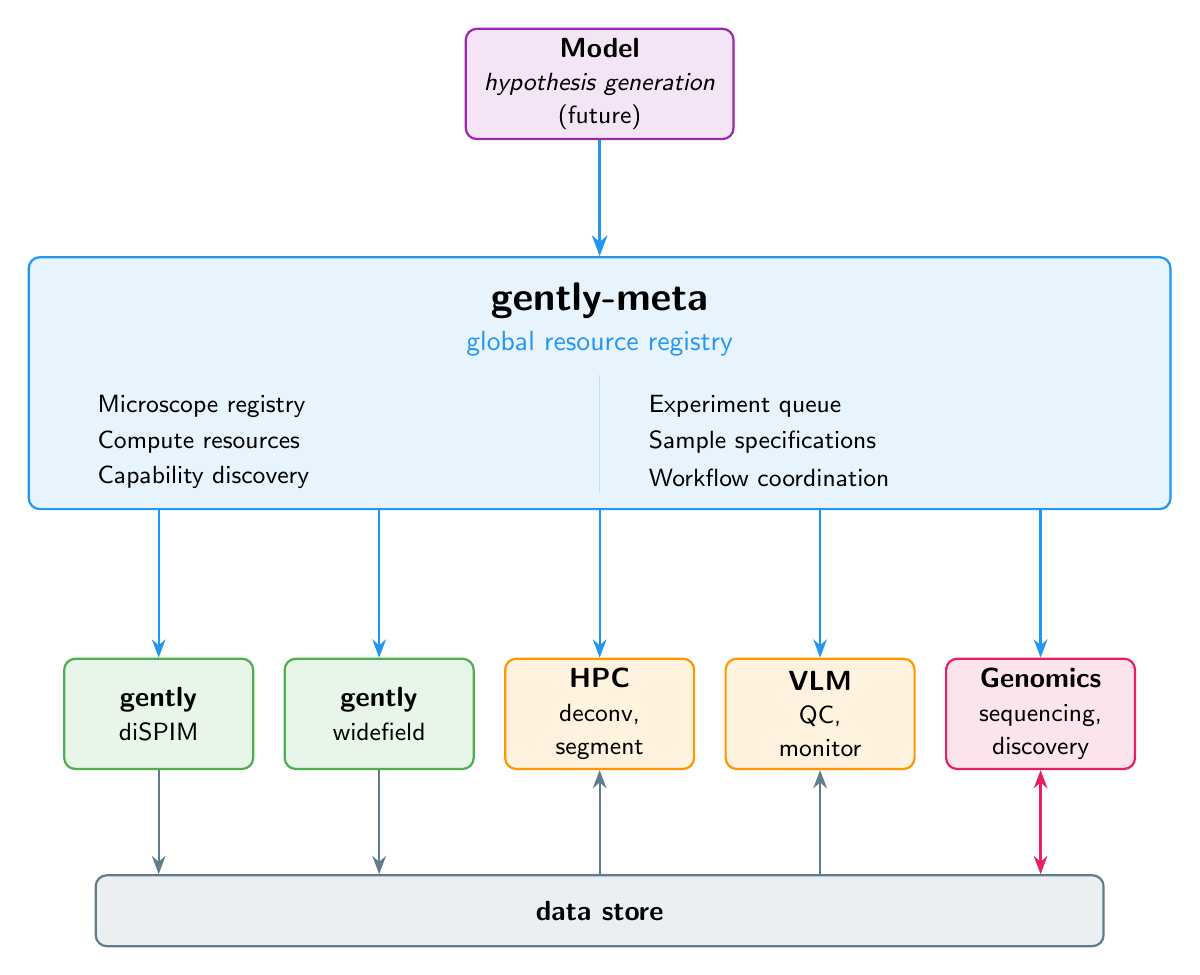
\begin{tikzpicture}[
    >=Stealth,
    every node/.style={font=\sffamily},
    box/.style={
        draw, rounded corners=4pt, minimum width=2.4cm,
        minimum height=1.4cm, align=center, line width=0.8pt
    },
    bullet/.style={font=\sffamily\small, anchor=west},
]

% Model node (top)
\node[box, fill=modelbg, draw=modelborder, minimum width=3.4cm] (model)
    at (0, 0)
    {\textbf{Model}\\\small\textit{hypothesis generation}\\\small (future)};

% gently-meta box
\node[box, fill=metabg, draw=metaborder, minimum width=14.5cm, minimum height=3.2cm]
    (meta) at (0, -3.8) {};

% Title and subtitle
\node[font=\sffamily\Large\bfseries] at (0, -2.75)
    {gently-meta};
\node[font=\sffamily, text=metaborder] at (0, -3.3)
    {global resource registry};

% Left column
\node[bullet] at (-6.5, -4.1) {Microscope registry};
\node[bullet] at (-6.5, -4.55) {Compute resources};
\node[bullet] at (-6.5, -5.0) {Capability discovery};

% Thin column separator
\draw[metaborder!30, line width=0.5pt] (0, -3.7) -- (0, -5.2);

% Right column
\node[bullet] at (0.5, -4.1) {Experiment queue};
\node[bullet] at (0.5, -4.55) {Sample specifications};
\node[bullet] at (0.5, -5.0) {Workflow coordination};

% Resource nodes
\node[box, fill=gentlybg, draw=gentlyborder] (dispim)
    at (-5.6, -8)
    {\textbf{gently}\\\small diSPIM};

\node[box, fill=gentlybg, draw=gentlyborder] (widefield)
    at (-2.8, -8)
    {\textbf{gently}\\\small widefield};

\node[box, fill=computebg, draw=computeborder] (hpc)
    at (0, -8)
    {\textbf{HPC}\\\small deconv,\\\small segment};

\node[box, fill=computebg, draw=computeborder] (vlm)
    at (2.8, -8)
    {\textbf{VLM}\\\small QC,\\\small monitor};

\node[box, fill=genomicsbg, draw=genomicsborder] (genomics)
    at (5.6, -8)
    {\textbf{Genomics}\\\small sequencing,\\\small discovery};

% Data store
\node[box, fill=storebg, draw=storeborder, minimum width=12.8cm, minimum height=0.9cm]
    (store) at (0, -10.5)
    {\textbf{data store}};

% Arrow: Model -> gently-meta
\draw[->, line width=1pt, metaborder] (model) -- (meta);

% Arrows: gently-meta -> resource nodes
\draw[->, line width=0.8pt, metaborder] (meta.south -| dispim) -- (dispim);
\draw[->, line width=0.8pt, metaborder] (meta.south -| widefield) -- (widefield);
\draw[->, line width=0.8pt, metaborder] (meta.south -| hpc) -- (hpc);
\draw[->, line width=0.8pt, metaborder] (meta.south -| vlm) -- (vlm);
\draw[->, line width=0.8pt, metaborder] (meta.south -| genomics) -- (genomics);

% Arrows: resources <-> data store
% Microscopes produce data
\draw[->, line width=0.8pt, storeborder] (dispim) -- (store.north -| dispim);
\draw[->, line width=0.8pt, storeborder] (widefield) -- (store.north -| widefield);
% HPC and VLM consume data
\draw[<-, line width=0.8pt, storeborder] (hpc) -- (store.north -| hpc);
\draw[<-, line width=0.8pt, storeborder] (vlm) -- (store.north -| vlm);
% Genomics bidirectional — produces discoveries, consumes imaging results
\draw[<->, line width=0.8pt, genomicsborder] (genomics) -- (store.north -| genomics);

\end{tikzpicture}
\end{document}
